\section{Introduction}
\subsection{Quantities of Interest}
In Epidemiological Studies, we want to measure the occurence. More specifically, we want to measure the \textbf{prevalence} and \textbf{incidence}.
\subsubsection*{Prevalence}
There are two measures of prevalence
\begin{enumerate}
    \item \textbf{Point Prevalence}: The proportion of at-risk population affected at a specific time \textbf{point}. Formally:
    \item \textbf{Period Prevalence}: The proportion of at-risk population affected at a specific time \textbf{period}.
\end{enumerate}
\subsubsection*{Incidence}
There are also two measures of incidence.
\begin{enumerate}
    \item \textbf{Incidence Proportion}: The proportion of a defined at-risk population who has affected within a specific time \textbf{point}.
    \item \textbf{Incidence Rate}: 
\end{enumerate}
\subsection{Association}
Association is \textbf{NOT} causation, it is the comparisions between groups.
\begin{definition}
    \textbf{Relative Risk} of an outcome Y with a binary risk factor A is:$$
    RR=\frac{P(Y=1 \mid A=1)}{P(Y=1 \mid A=0)}
    $$
    where $0<RR<\infty$
\end{definition}
Note that:
\begin{enumerate}
    \item $P(A=1)+P(A=0)=1$
    \item $RR=1\implies Y=1 \perp A=1\implies\text{No association between Y and A}$
    \item $
    \text {If } RR>1 \text {, there is greater risk of } Y=1 \text { when } A=1 \text { vs } A=0, vice-versa
    $
    \item $\frac{P(Y=1 \mid A=1)}{P(Y=1 \mid A=0)}\neq \frac{P(A=1 \mid Y=1)}{P(A=1 \mid Y=0)}$
\end{enumerate}
\begin{definition}
    \textbf{Odds Ratio}\par
    \begin{itemize}
        \item The odds of a disease $Y$ among the exposed $A=1$

        $$
        \left.=\frac{P(Y=1 \mid A=1}{P(Y=0 \mid A=1)}\right)=\frac{P(Y=1 \mid A=1)}{1-P(Y=1 \mid A=1)}
        $$
        
        \item The odds of disease $Y$ among the unexposed $A=0$
        
        $$
        =\frac{P(Y=1 \mid A=0)}{P(Y=0 \mid A=0)} \frac{P(Y=1 \mid A=0)}{1-P(Y=1 \mid A=0)}
        $$
        
        \item The odds ratio for measuring the association of disease with the exposed vs. unexposed groups is:        
        \begin{align*}
            OR & =\frac{P(Y=1 \mid A=1) / P(Y=0 \mid A=1)}{P(Y=1 \mid A=0) / P(Y=0 \mid A=0)}\\
            &=\frac{P(Y=1 \mid A=1) /[1-P(Y=1 \mid A=1)]}{P(Y=1 \mid A=0) /[1-P(Y=1 \mid A=0)]}\\
            &=\underbrace{\frac{P(Y=1 \mid A=1)}{P(Y=1 \mid A=0)}}_{RR}\times\frac{P(Y=0 \mid A=0)}{P(Y=0 \mid A=1)}
        \end{align*}        
    \end{itemize}
\end{definition}
Note that:
\begin{enumerate}
    \item $OR=1\Leftrightarrow log(OR)=0\:\text{means no association between}\:Y\:\text{and}\:A$
    \item $OR\leq 1\:\text{means greater odds of ratio when exposed}$
    \item The OR for Y given A is equal to the OR for A given Y$$
    OR=\frac{\frac{P(Y=1 \mid A=1)}{P(Y=0 \mid A=1)}}{\frac{P(Y=1 \mid A=0)}{P(Y=0 \mid A=0)}}=\frac{\frac{P(A=1 \mid Y=1)}{P(A=0 \mid Y=1)}}{\frac{P(A=1 \mid Y=0)}{P(A=0 \mid Y=0)}}
    $$
    \item OR is a goods estimate of RR for rare disease as the second term above will approximate to 0.
    \item $RR>1\implies OR>RR,\:RR<1\implies OR<RR$
\end{enumerate}
\begin{definition}
    \textbf{Risk difference}\\
    $$
    RD=P(Y=1 \mid A=1)-P(Y=1 \mid A=0)
    $$
    where $-1<RD<1$
\end{definition}
This can be understood as the additional risk when exposed. In addition, a positive $RD$ means a greater risk when exposed, vice-versa.
\begin{definition}
    \textbf{Attributable Risk(AR)}\\
    AR is the fraction of the cases of the outcome $Y=1$ that can be attributed to $A=1$
    $$
    AR=\frac{P(Y=1)-P(Y=1 \mid A=0)}{P(Y=1)}
    $$
    Furthermore:
    \begin{align*}
    AR&=\frac{P(A=1)[P(Y=1 \mid A=1)-P(Y=1 \mid A=0)]}{[P(Y=1 \mid A=1) P(A=1)]+[P(Y=1 \mid A=0) P(A=0)]}\\
    &=\frac{P(A=1)[R R-1]}{[P(A=1) R R]+P(A=0)}=\frac{P(A=1)[R R-1]}{(P(A=1)[R R-1])+1}
    \end{align*}
    We can see that the $AR$ depends on both the association between $A$ and $Y$ via $RR$, and the prevalence of risk factor at $A=1$
\end{definition}
Note that:
\begin{enumerate}
    \item $ AR=0 \Longleftrightarrow RD=0 \Longleftrightarrow O R=1 \Longleftrightarrow R R=1 $ is null, meaning that $A\perp Y$
    \item $AR>0$ means the A will rise the risk of Y; $AR<0$ means A is protective, decrease the risk of Y.
    \item $AR$ does not imply causation.
\end{enumerate}
\subsection{Causation}
Two variables are causally related if changing one can potentially change the level of the other. In causal inference, \( A \) represents the treatment, where \( A=1 \) stands for the exposed or treated group, and \( A=0 \) represents the unexposed or control group. The variable \( Y \) is the observed outcome.

In contrast, we also have the concept of the \textbf{potential outcome}, which captures the outcome under different treatment conditions.
\begin{definition}
    \textbf{Potential Outcome and Individual Causal Effect (ICE)}\\
    The potential outcome framework includes outcomes that may or may not be observed. More specifically:
    \begin{itemize}
        \item \( Y^0 \) (or \( Y(0) \)) is the potential outcome if assigned to the control group (\( A=0 \)).
        \item \( Y^1 \) (or \( Y(1) \)) is the potential outcome if assigned to the treatment group (\( A=1 \)).
    \end{itemize}
    Importantly, in reality, only one of \( Y^0 \) or \( Y^1 \) is observed for any individual; the other is counterfactual. This is also called the \textbf{Foundamental Problem}.\\
    
    The \textbf{Individual Level Causal Effect (ICE)} is defined as:
    \[
    ICE = Y^1 - Y^0
    \]
\end{definition}

Since we can only observe one of \( Y^1 \) and \( Y^0 \) for any individual, this is known as the \textbf{consistency assumption}. Formally, the observed outcome \( Y \) is represented as:
\[
Y = A Y^1 + (1 - A) Y^0 \quad \text{or} \quad Y = Y^A
\]
This implies that an individual cannot belong to both the treatment and control groups simultaneously. However, an individual can receive different treatments at different time points.

\begin{remark}
    \textbf{Stable Unit Treatment Value Assumption (SUTVA)}\\
    The consistency is implied by the \textbf{Stable Unit Treatment Value Assumption (SUTVA)}, which consists of two key conditions:
    \begin{enumerate}
        \item \textbf{No interference}: The outcome of one individual is not affected by the treatment status of other individuals.
        \item \textbf{Well-defined treatment}: There is a single version of the treatment; no multiple versions of the treatment exist.
    \end{enumerate}
\end{remark}
\begin{definition}
    \textbf{Average Causal Effect (ACE)}\\
    To solve the foundamental problem, instead of using ICE, we take ACE.
    \begin{align*}
        ACE&=E\left[Y^1-Y^0\right]\\
        &=E\left[Y^1\right]-E\left[Y^0\right]\\
        &=1\times P[Y^1=1]+0\times P[Y^1=0]-(1\times P[Y^0=1]+0\times P[Y^0=0])\\
        &=P\left[Y^1=1\right]-P\left[Y^0=1\right]
    \end{align*}
\end{definition}
\subsection{Association vs. Causation}
\begin{remark}
    $E[Y^1]\neq E[Y|A=1]$
    \begin{itemize}
        \item $E\left[Y^1\right]$ is a priori, and is the average value defined by the \textbf{entire population}.
        \item $E[Y \mid A=1]$ is defined after treatment assignment, and averaged only \textbf{among} those who receive treatment $A=1$.
        \item We use $E\left[Y^1\right]$ in Causation and $E[Y \mid A=1]$ in Association.
    \end{itemize}
\end{remark}

\begin{figure}
    \centering
    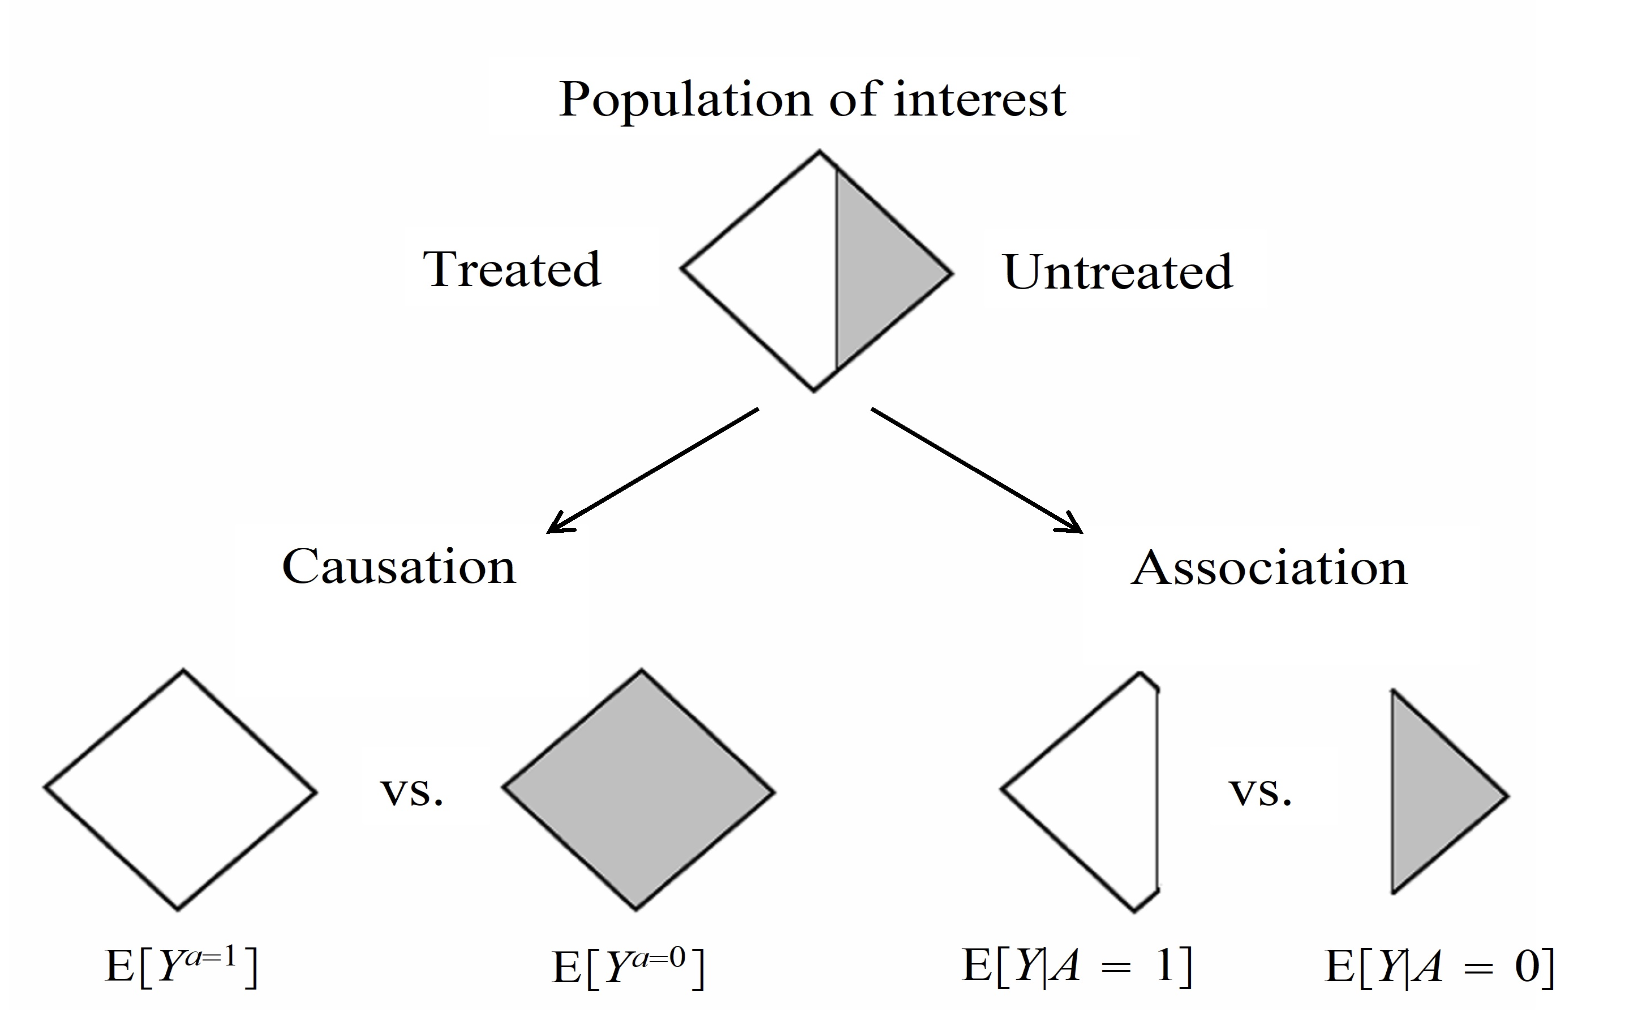
\includegraphics[width=.7\linewidth]{codes/figures/section1/figure_1_1.png}
    \caption{Visualization of Association and Causation}
    \label{fig:as_ca}
\end{figure}
\hyperref[fig:as_ca]{Figure 1.1} visualizes the difference between association and causation. Moreover, like discussed above, we also have causal \textbf{Risk Ratio}, causal \textbf{Odds Ratio} and causal \textbf{Risk Difference}.
\begin{definition}
    \textbf{Measures of Causal Effect}\\
    \begin{enumerate}
        \item \textbf{Causal Risk Ratio}
        $$
        R R=\frac{P\left(Y^1=1\right)}{P\left(Y^0=1\right)}
        $$
        
        \item \textbf{Causal Odds Ratio}
        $$
        O R=\frac{P\left(Y^1=1\right) /\left[1-P\left(Y^1=1\right)\right]}{P\left(Y^0=1\right) /\left[1-P\left(Y^0=1\right)\right]}
        $$

        \item \textbf{Causal Risk Difference}
        
        $$
        R D=P\left(Y^1=1\right)-P\left(Y^0=1\right)
        $$
    \end{enumerate}
\end{definition}
\begin{remark}
    \textbf{Summary of Association vs. Causation}\\
    \begin{tabular}{p{7cm} p{7cm}}
        \textbf{1. (Associational) Risk Ratio} &
        \textbf{1. Causal Risk Ratio} \\
        \[
        RR = \frac{P(Y = 1 \mid A = 1)}{P(Y = 1 \mid A = 0)}
        \] &
        \[
        RR = \frac{P(Y^1 = 1)}{P(Y^0 = 1)}
        \] \\
        \textbf{2. (Associational) Odds Ratio} &
        \textbf{2. Causal Odds Ratio} \\
        \[
        OR = \frac{\frac{P(Y = 1 \mid A = 1)}{1 - P(Y = 1 \mid A = 1)}}{\frac{P(Y = 1 \mid A = 0)}{1 - P(Y = 1 \mid A = 0)}}
        \] &
        \[
        OR = \frac{\frac{P(Y^1 = 1)}{1 - P(Y^1 = 1)}}{\frac{P(Y^0 = 1)}{1 - P(Y^0 = 1)}}
        \] \\
        \textbf{3. (Associational) Risk Difference} &
        \textbf{3. Causal Risk Difference} \\
        \[
        RD = P(Y = 1 \mid A = 1) - P(Y = 1 \mid A = 0)
        \] &
        \[
        RD = P(Y^1 = 1) - P(Y^0 = 1)
        \]
    \end{tabular}
    
\end{remark}

The \textbf{Sharp Null/Causal Null} (for ACE) means no causal effect; equivalently $AR=0 \Longleftrightarrow RD=0 \Longleftrightarrow OR=1 \Longleftrightarrow RR=1$. However, holding sharp null for ACE does \textbf{NOT} necessarily mean the sharp null for individual causal effect also holds.